\chapter{Analytics in use}~\label{chapter-analytics-in-use}

This chapter presents the research findings based on two of the six perspectives: \uuse and \iuse, \emph{i.e.} how app developers currently use mobile analytics and ways the use could be improved. Figure \ref{fig:dev-practices-with-mobile-analytics} provides the visual context of the development practices and artefacts~\footnote{This figure will be revised pre-submission and keyed into the contents of this chapter. Versions of this figure may feature throughout the thesis with the pertinent elements highlighted and less relevant elements diminished or hidden from view.}.

\begin{figure}
    \centering
    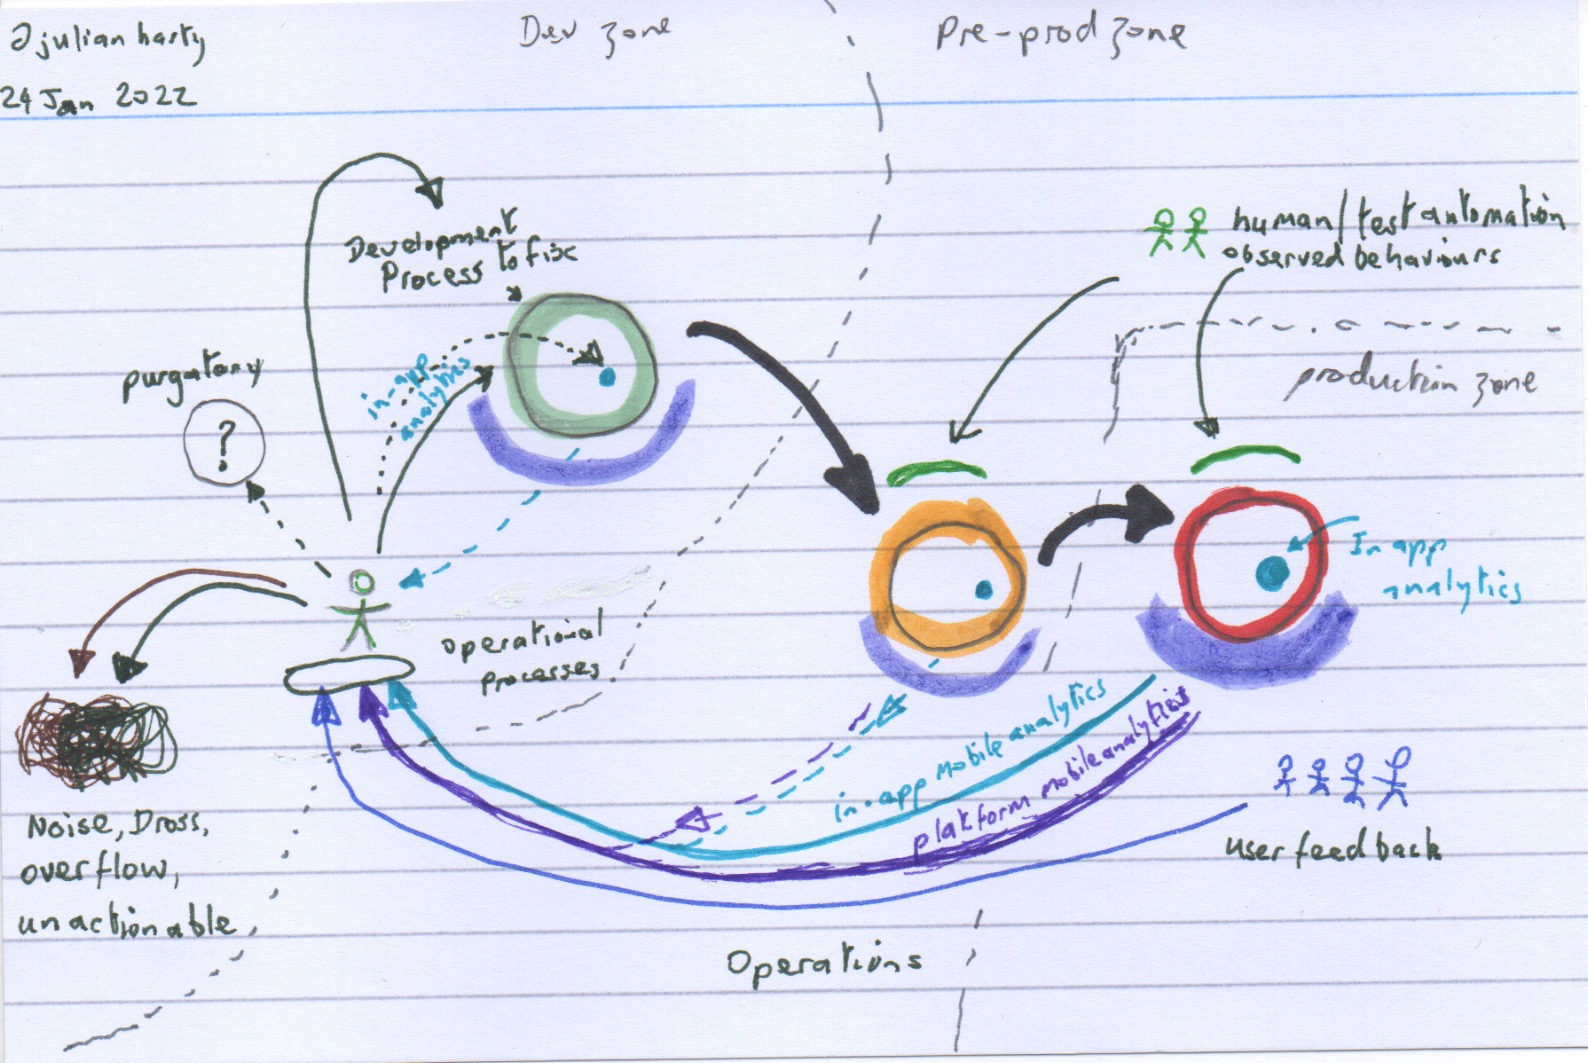
\includegraphics[width=12cm]{images/rough-sketches/dev-practices-with-mobile-analytics-24-jan-2022.jpeg}
    \caption{Dev Practices with Mobile Analytics}
    \label{fig:dev-practices-with-mobile-analytics}
\end{figure}

\julian{TODO introduce the rest of this chapter. Here's my current running order: \href{aiu-motivating-factors-section}{Motivation}, \href{aiu-choosing-mobile-analytics-section}{selection}, \href{aiu-application-of-mobile-analytics-section}{application}, 
\href{aiu-bug-reproduction}{bug reproduction}, 
\href{aiu-triage-section}{triage}, 
blockers,  
\href{aiu-snafu-and-real-world-conditions-section}{snafu and real-world conditions}, 
\href{aiu-integration-section}{integration}, 
\href{aiu-engineering-tradeoffs-section}{engineering tradeoffs},
the~\href{aiu-discussion-section}{discussion}}

\section{Motivating factors}~\label{aiu-motivating-factors-section}
What motivates the development teams to pay attention and address failures reported by mobile analytics? The motivation may be viewed as a bi-directional continuum: at one end there is the wish to avoid and restrict failures that affect end users of the apps, at the other end there are desires to improve apps, engineering practices, including improving the use of mobile analytics. Fixing failures may be more tactical, while desiring improvements may be more strategic and involve a longer-term perspective.

In terms of the app-centric case studies only one of the interview-based studies - \href{glossary-gtaf}{GTAF} - explicitly explained they had periods of fixing high crash rates. Several of their Android apps had experienced high crash rates which had adversely affected the user experience. The project team have learned the importance of paying attention to crashes being reported by mobile analytics tools. They also realised the importance of addressing high crash rates. Accordingly, the development team used outputs from mobile analytics to identify the most frequent crashes they wanted to fix. In contrast, the majority of the rest of the interview-based studies were predominantly working to maintain good quality, to varying degrees based on their active and ongoing use of mobile analytics. The one odd-ball project was LocalHalo where the CTO appeared to only use mobile analytics infrequently despite having actively integrated several in-app analytics tools into their app and server codebases.

All of the action research-based app centric case studies were prompted by excessively high crash rates \emph{i.e.} they acknowledged they wanted/needed help both to tame the high crash rates and to improve the rates further on an ongoing basis.

For Kiwix, there was a pernicious, insidious increase in the crash rates for several of the most popular Android apps. The project leads particularly wanted to reduce the crash rates for the worst offenders in terms of the apps. Similarly the crash rate for Pocket Code far exceeded the bad behavior threshold, of 1.09\%, and despite the various recommended software development practices the project team had not been able to tame the excessive crash rate.

For the commercial app, it had a user-base of millions however bouts of issues in several releases of the Android app meant the app had significantly exceeded the bad behavior threshold, of 1.09\%, Google applies to all Android apps in the Google Play Store. They needed to solve the tactical issues in parallel with improving the engineering practices to reduce the likelihood of similar bouts and to encourage ongoing and long-lasting improvements to the quality of their app and the service. 

The commercial app-centric case studies all incorporated general purpose usage analytics into their apps in addition to error reporting, Firebase Analytics was the most popular choice, which is congruent with Firebase Analytics being the dominant market leader~\citep{appbrain_firebase}. LocalHalo chose Sentry, in part as it integrated well with React-Native, the cross-platform development framework they used for their mobile app.

The use of additional general purpose analytics is not confined to the commercial apps, Greentech apps team demonstrated how they had actively used mobile analytics to reduce the crash rate of their key apps and announced their intention to increase their use of mobile analytics in order to improve the user experience of their apps~\citep{gtafblog2021_gtaf_accomplishment_2020}. 

An interesting example from grey literature is the use of an error budget where the developers have 20\% of their time available to work on technical improvements. If the app's crash free rate is above 99.9\% the team can choose their work freely, however when the crash rate exceeds 0.1\% then the developers must spend their 20\% fixing the problem (described as the situation in the literature)~\citep{koutun2021_how_to_deal_with_tech_debt_at_the_scale_of_super_app}.

\section{Choosing Mobile Analytics}~\label{aiu-choosing-mobile-analytics-section}

\julian{TODO expand on selection and choosing}
The choice of which mobile analytics tools to use is in some ways a recursive characteristic. Firstly, there is the choice of whether to include any analytics within the app at all - the Kiwix project team chose not to in order to maximise the protection of end users' privacy and minimise the potential for repressive authorities finding and then abusing usage-related data to penalise end users of Wikipedia and similar material. The rest of the app-centric case studies included at least one in-app mobile analytics SDK in their app.

Some of the projects, including LocalHalo, Greentech apps, and the Commercial project, choose to incorporate several mobile analytics SDKs in their apps. Their reasons differed, for example LocalHalo used Mixpanel for business analytics and Sentry for technology-related analytics including crash reporting. Greentech apps appears to let each app developer decide on which mobile analytics service to incorporate. The corporate projects reasons were multi-factoral and outside the scope of the research.

Choices of SDK may change over time: for example the Catrobat project chose to remove in-app analytics from their flagship Pocket Code app as the replacement for the Fabric Crashlytics SDK also collected and combined PII data with the crash reporting. Like the Kiwix project team they wanted to err on protecting the privacy of their users (which includes many school-age children) and reduce their contributions to the already vast digital footprint owned by global tech superpowers.

Secondly, there is the choice of which source to use for which purposes. For instance both Android Vitals and the many crash reporting SDKs report on app crashes. All the projects who used in-app mobile analytics for crash reporting preferred to use that service to monitor the crashes in their app, even if some crashes aren't reported in that tool, for example those that occur as the app is starting up. Of the development teams who used in-app crash reporting Moonpig were unusual as they \textit{also} actively and frequently used Android Vitals to monitor crashes and other failures.

Thirdly, there are choices to be made in terms of what to record and when to do so in terms of in-app mobile analytics. Various in-app mobile analytics SDKs provide facilities for error reporting in addition to crash reporting. Broadly errors in this context are connected to caught and handled Java exceptions~\footnote{For avoidance of doubt this includes Kotlin and other JVM languages, errors reported in frameworks such as React Native, and caught signals in C++ code.}. Some SDKs include API calls to provide trails of `breadcrumbs' that lead up to an error or a crash~\footnote{For instance, see \url{https://www.bugsnag.com/blog/android-breadcrumbs-support}.}. None of the app-centric case studies mentioned actively using these breadcrumbs, however the reports Sentry generated for the LocalHalo app indicate the Sentry SDK generated automatic breadcrumbs~\footnote{\url{https://docs.sentry.io/platforms/react-native/enriching-events/breadcrumbs/}} and these helped identify the server was no longer functioning correctly in late 2021. 

%%%% Sources include: 
%%%%%%% https://www.bugsnag.com/blog/error-handling-on-android-part-7 
%%%%%%% https://github.com/backtrace-labs/backtrace-android
%%%%%%% https://backtrace.io/
%%%%%%% https://saucelabs.com/platform/error-reporting (which also mentions triage)
%%%%%%% For breadcrumbs several are listed in https://www.google.com/search?q=breadcrumb+crash+reporting+android 

Caught exceptions, signals, etc. are not the only form of error that might be of interest to developers. Projects including Smartnavi and Moonpig used general purpose mobile analytics for reporting additional errors, for instance that affected the user experience. Similarly the general purpose mobile analytics and the crash reporting SDKs both collect contextual and runtime information and developers sometimes use this information. Some additional joint research studied 107 actively maintained opensource Android apps hosted on GitHub, a topic we cover shortly\pending{TODO}.

But before we move on there was an interesting phenomenon observed during the Catrobat hackathon where some of the crashes that appeared in Android Vitals were believed to come from `soft errors' in the Pocket Code app. The issue, CATROID-426, was logged during the hackathon~\citep{catroid_426_soft_crashes_should_not_be_reported_to_the_play_console} and the developers wrote two sets of code changes (also known as `commits'). These were merged into the app's codebase on \nth{21} Nov 2019 and released in the pocket code several weeks later.

The intent was laudable, however, at least some of the soft crashes continued to occur over a month later, as documented in \url{https://jira.catrob.at/browse/CATROID-422}. This issue was raised in the hackathon and closed as a duplicate by one of the developers involved in trying to stop the soft errors from appearing in Android Vitals \citep{catroid_426_soft_crashes_should_not_be_reported_to_the_play_console}.

\subsection{Developer-controlled characteristics}
\julian{TODO expand on the following:}
TODO discuss the initial config, and `getting started', then the optional additional use of the mobile analytics SDK's APIs. Provide examples from the log analysis research where 50 of 107 projects only used the minimal default initialisation rather than calling the rest of the Firebase Analytics API. 

TODO Mention the Pocket Code experience when migrating from Fabric to Firebase and the additional, unexpected analytics that appeared. Forward reference to the discussion on intrusiveness. 


\section{Application of mobile analytics}~\label{aiu-application-of-mobile-analytics-section}

\julian{Include horses-for-courses,...} 
As mentioned previously, several projects including LocalHalo chose to use a particular mobile analytics service for   business analytics. Pricing may also be a factor in the choice of SDK and service, however this topic was not actively discussed as part of the case studies.

\section{Bug reproduction}~\label{aiu-bug-reproduction}
Being able to reproduce bugs, ideally at-will, enables developers to work more effectively at addressing the bug and having confidence that their intended fixes actually do fix the bug. 
Bug reproduction can increase the developer's confidence the bug is real and can be managed, it is under control. Then they can make changes to the the software to determine whether their changes address (fix) the bug. 

The developers are not always able to reproduce bugs, for example the developers of the Pocket Code app had to apply their `fix' blindly with the immediate aim of fixing, \emph{i.e.} preventing, the crash \url{https://github.com/Catrobat/Catroid/pull/3362}.  In the commercial app, two experienced engineers spent several days in devising a consistent and clear way to reproduce a crash in the response handling and logging for proprietary code that interacted with the very popular OkHttp opensource library. This effort was deemed necessary and appropriate given the strategic importance of the app to the business and the effects of the crash on a significant subset of users' sessions.

The research also had mixed results reproducing bugs that were found and reported by mobile analytics.
%
The Kiwix project included crashes in several software components Google provides android developers: the WebView (an embedded browser), and Chrome.apk - the binary file for the Google Chrome Android app. It also included attempts to reproduce crashes in the app's codebase. 

\begin{itemize}
    \item One experiment used the same model of Samsung Android smartphone that incurred a higher than usual crash rate, however there was insufficient information available in Android Vitals to determine enough of the events that led to the crash or any of the contextual information. The manual interactive testing did not manage to reproduce the crash.
    \item Another experiment scripted the semi-autonomous Android Monkey testing utility where the script seeded each test run to make the sequence of generated inputs consistent with the aim of first triggering crashes and then having sufficient information to reproduce those crashes at will.
    \item Note: a third experiment was on hold for several years awaiting availability of the software tool, CrashScope. This became available in late 2021 and the testing is pending the configuration of the tests with the various apps.
\end{itemize}

With the exception of the Commercial project, none of the commercial projects (Moonpig, Moodspace, LocalHalo) provided examples of being able to reproduce crashes and other failures that were reported by mobile analytics; nonetheless they chose to use in-app analytics and the respective mobile analytics reports in preference to Android Vitals as they believed these tools provided more relevant reports with the necessary information to enable the developers to find and fix the causes of those crashes.

\section{Triage}~\label{aiu-triage-section}
\julian{Include decision making, adverse side effects (which feeds into snafu and real-world conditions).}

The Triage is where the developers decide what to do, if anything, with failure clusters being reported by mobile analytics. Several of the projects confirmed used mobile analytics as a source when the issues are triaged and the others \textit{probably} did so too even though it was not discussed explicitly.

Broadly the triage process results in one of four outcomes:
\begin{enumerate}
    \item Accepted issues: which the project team intend to address.
    \item Pending issues: where the project team need more information before being able to reach a triage decision.
    \item Explicitly rejected issues: those the developers actively chose not to action, for instance as those impractical to address. Note: Some mobile analytics tools provide a facility for developers to ignore or mute these issues.
    \item Implicitly rejected issues: for some projects this applies to the majority of the failures reported by the various mobile analytics tools.
\end{enumerate}

The triage process sometimes led to issues being raised in the respective issues database for at least some of the issues they chose to action, for example Catrobat reported them in JIRA, Greentech Apps use GitLab's integrated issues database, Kiwix similarly use Github issues\pending{Ask Moonpig what they did} and the commercial app used recorded them in their organisation-wide issues database. However, projects did not necessarily record every such actioned issue. 

\newthought{Triaging failures}

\newthought{Hard to fix issues}
The GTAF team used a heuristic when deciding which crashes to fix. They chose to work on those perceived as relatively easy to fix and which affected many users. They provided examples of easier to fix exceptions: NullPointerException~\footnote{Helpfully discussed in \href{https://en.wikibooks.org/wiki/Java\_Programming/Preventing\_NullPointerException}{en.wikibooks.org/wiki/Java\_Programming/Preventing\_NullPointerException}.} and IndexOutOfBoundsException~\footnote{Discussed in \url{https://stackoverflow.com/a/40006381/340175}} versus some they found harder to fix: IllegalStateException~\footnote{An example of an Android specific crash is discussed in~\url{https://stackoverflow.com/questions/55158930/illegalstateexception-caused-by-intent}} and native crashes~\footnote{Useful Android documentation on diagnosing native crashes \url{https://source.android.com/devices/tech/debug/native-crash}}.


\section{SNAFU and real-world conditions}~\label{aiu-snafu-and-real-world-conditions-section}
Software development, including developing apps, takes place in the real-world where there are often multiple conflicting demands on the time of participants - the developers. Therefore, absolutes, superlatives, and other pure approaches are unlikely to work. Bugs will happen, automated tests, if written at all, won't necessarily test much or test in depth, \xcancel{bugs will happen}, nothing will be perfect.

The impracticality of perfection leads to real-world consequences, to coping strategies, to pragmatic behaviours, and so on. There's a term, snafu~\footnote{\url{https://en.wikipedia.org/wiki/SNAFU}}, Several examples of snafu emerged in terms of a) developing apps, b) in the development teams using mobile analytics, and c) an accidental misconfiguration pre-release that led to a mute release of Pocket Code.

Firstly, in terms of developing apps, there is poor reliability of the apps in use by default. Kiwix, Catrobat, Greentech Apps, and the Commercial project all had ongoing periods where the reliability was excessively poor and beyond one or more of Google's Bad Behavior Thresholds~\citep{play_console_help_android_vitals_2019}. Indications from the evidence gathered is poor reliability accretes when developers do not actively monitor mobile analytics and address the more severe of the failures that are reported. Conversely when developers do address these failures the reliability of the subsequent release of the app generally increases - a topic discussed in the next chapter.

Another snafu factor is when developers do not have access to mobile analytics outputs, or when they do have access but they are not able to use the outputs productively. As access to the mobile analytics tools is restricted by default~\footnote{At least access has been restricted for every tool and service that feature in this research.} someone has to grant access to the particular individual developer. For projects where one person plays all the roles that person will have access as they are the account owner, Moodspace is a good example here. For LocalHalo only the CTO and the researcher had access to Sentry, it is not clear why the rest of the development team lacked access.

Especially for larger teams, and teams where participation is periodic, many team members are not granted access. Three of the app-centric case studies exemplify this: Catrobat, Kiwix, and the Commercial Project. Conversely, all the developers at Moonpig are provided with at least read access to Google Play Console with Android Vitals and to Firebase Analytics.

The third example of snafu is for the Pocket Code project. An accidental misconfiguration during the release process led to the loss of Fabric Crashlytics data for that release. Fortunately, Google Play Console with Android Vitals continued to provide ongoing outputs indicating the benefits of having platform-level mobile analytics. The development team applied the correct configuration for the following release of the app and Fabrics Crashlytics data was restored for subsequent releases.

\subsection{Engineering tradeoffs}~\label{aiu-engineering-tradeoffs-section}

Kiwix download code substitution, positive effects, knock-on effects in terms of functionality.
Perceived maintenance overhead of making interim releases of the app meant the dev leads rejected the proposal \url{https://github.com/kiwix/kiwix-android/issues/1426}. A secondary consideration is the burden of creating and rolling out releases of the custom apps; at the time the release process was burdensome for the developers. 

Moonpig took several months to first replace the Robospice SDK and then deploy the new release without that library. Release management is a key factor in decision making. Crash analytics helped quantify the effects on groups of affected users (those on newer releases of Android).

Flo Health have explicit tradeoffs between how developers spend their time developing their app. Firstly they only spend 80\% of the time on core development, the remaining 20\% is ring-fenced for other development work. This 20\% is either spent on whatever the developers choose to work on, or on addressing errors if any error budget has been exceeded~\citep{koutun2021_how_to_deal_with_tech_debt_at_the_scale_of_super_app}.

\newthought{Release management}
Two examples of release management have already been mentioned (for Kiwix custom apps and for Moonpig), the Commercial Project also placed great importance on scheduling releases with the intention of maintaining the goodwill and encouraging adoption of the new release. 

Google Play Console incorporates various aspects of its reports including various pre-filtered reports from Android Vitals into a Release Management section of the online GUI. The Release Management also includes mechanisms to perform a Staged Rollout which is particularly pertinent for apps with large userbases where it helps the development team to obtain focused information about the reliability and the adoption of the new release while also constraining the risk of a release failing in production~\footnote{An overview of the Release Management features launched in Summer 2020 are covered in a short video \url{https://www.youtube.com/watch?v=vyReHI1eSSU}.}. 

The product owners for the Commercial Project learned about how to combine the Release Management reports (including Android Vitals aspects in particular) and Microsoft App Center's reports in order to have greater insights into the vital signs and overall health of new releases. Android Vitals was seen to provide fast feedback into the health of a series of releases of the Android app and it was a highly effective early warning indicator of reliability issues emerging in a new release. Of note, staged rollouts cannot be reduced, nor can staged rollouts be targeted to users of a particular release of the app, so it's not currently practical to perform incisive upgrades to replace a failing release without also upgrading some portion of the other users of the app.

\subsection{Sensemaking and decision-taking by developers}~\label{aiu-sensemaking-and-decision-taking-by-developers-section}
Beacon-finding and drill-down parallel similar practices used by app developers when they use mobile analytics as inputs to their development work and as feedback for [their] previous development work.

\begin{figure}
    \centering
    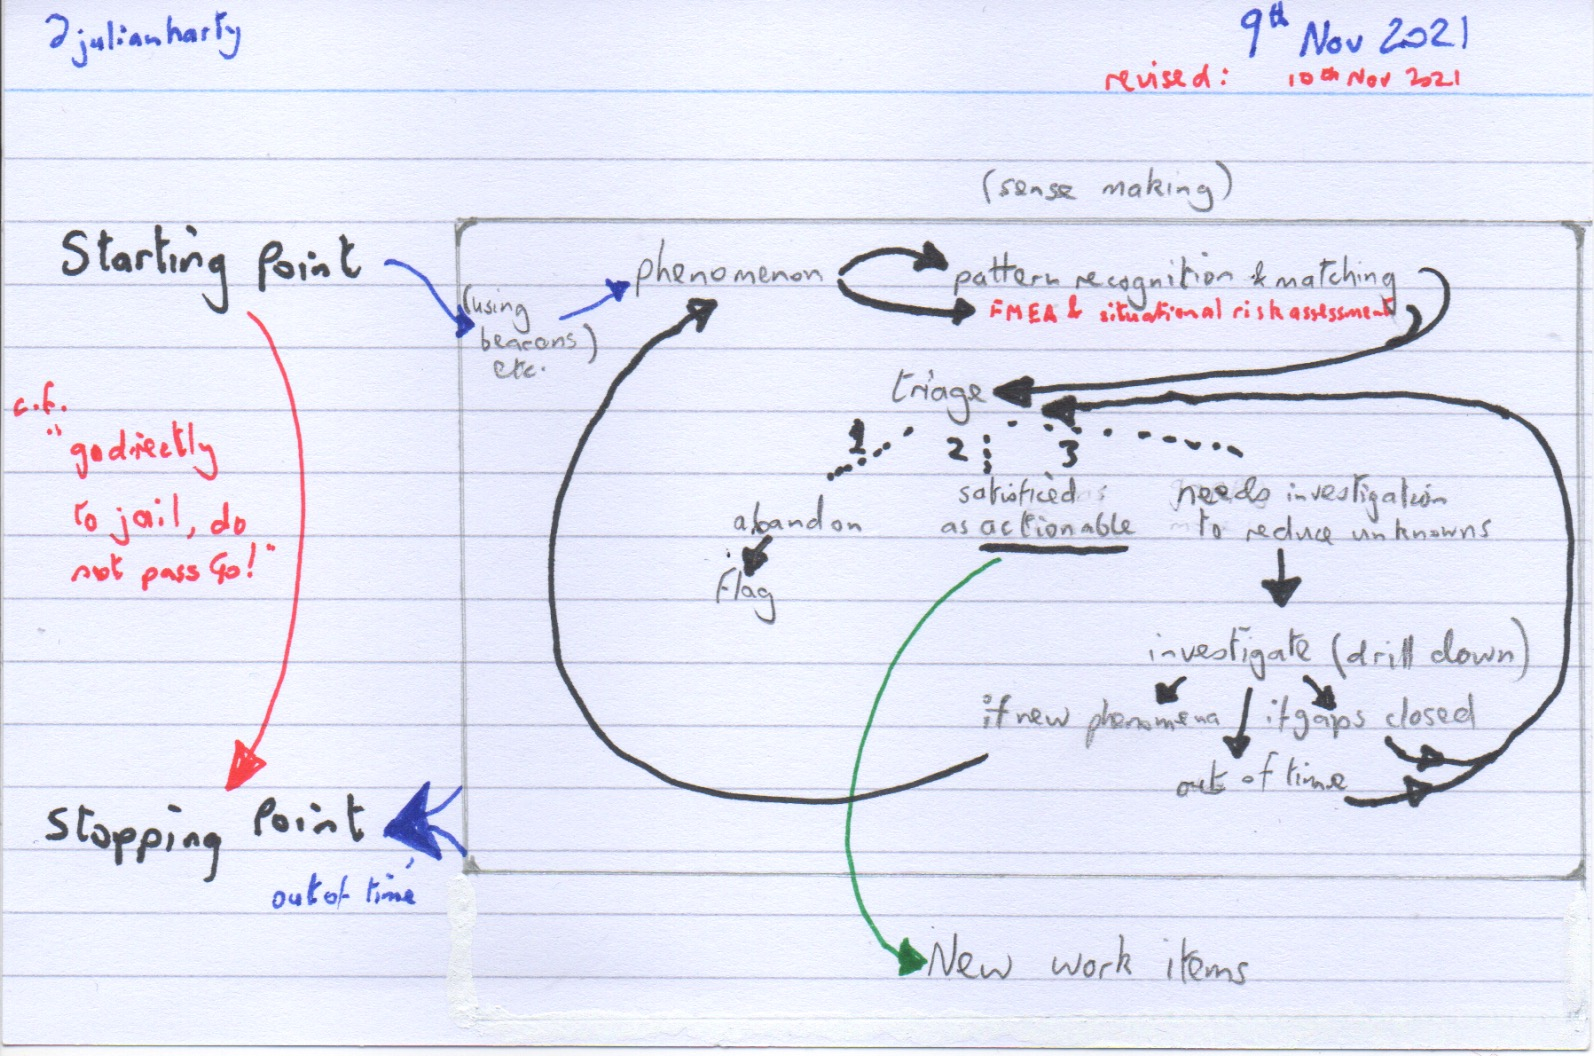
\includegraphics[width=15cm]{images/rough-sketches/practical-sense-making-process-10-nov-2021.jpeg}
    \caption{Sense-making process when development teams apply mobile analytics}
    \label{fig:practical-sense-making-process-when-dev-teams-apply-mobile-analytics}
\end{figure}


Figure~\ref{fig:practical-sense-making-process-when-dev-teams-apply-mobile-analytics} illustrates the sense-making and triage process used by development teams which shares various similarities with sense-making from a research perspective. These similarities mean the researcher and the practitioner may also share similar practices in terms of their analysis of phenomena found in mobile analytics tools. The triage and drill-down may be repeated several times where there is sufficient potential value in performing further investigation. 

The impact of reported failures is combined with situational-risk-assessment as a part of the decision-making process performed by developers during triage; for instance to consider whether this reported issue is worth addressing in the current development cycle, (\textit{e.g.} in the current sprint for teams who use sprints for work planning. Developers have to consider multiple criteria including personal, project, and product implications of making code and/or operational changes. An untested hypothesis for their approach is introduced in the discussion chapter on page \pageref{discussion-decision-making-by-dev-teams-section}.

\newthought{Premature satisfaction}

A possible suggestion, an inference, is that many of the developers were often satisficed with what the mobile analytics tools reported - where they accepted local optima (determined through a combination of observation and asking the app devs), \textit{e.g.} they accepted the `top' crash cluster as the worst one. Therefore, if there are flaws in what is being reported the effects of those flaws may permeate into the results of what the developers \textit{do} and \textit{don't} do. 

Indeed, as \secref{chapter-tools-and-their-artefacts} discusses\pending{Add more precise x-reference once that chapter has been fleshed out.} there are flaws in the groupings of similar failures in at least three of the mobile analytics crash reporting outputs.


\section{Integration}~\label{aiu-integration-section}
\julian{Include pipelines, tracking the source of issues including re-visiting integration into the triage process, trusting the tools, ...}

Integration in this context facilitates and improves the `working together' of mobile analytics with other software tools. It ranges from manual and often short term mechanisms to streamlined pipelining of mobile analytics outputs into other systems. Often there's a basic facility provided which enables issues to be raised directly from a mobile analytics web page.

As can be observed in the Greentech project's issues database, for example, the developers include the URL that points to the pertinent report in the source mobile analytics service. These links work for a period, typically hours to weeks, and are limited to people who have access to both systems. They enable authorised users to quickly check the source material from the relevant issue. 

These links eventually decay once the source content is no longer available. In the three main action research projects screenshots together with pertinent text-based extracts were included in the issues database to help preserve the information indefinitely. Similarly Vitals Scraper was developed and used to automate the collection of screenshots and the underlying data from Android Vitals to preserve the information and make it available for additional analysis.

Microsoft App Center, for example, has the facility where comments can be added to failure clusters. In the Commercial Project, for example, the developers often added a key in the comment field to indicate this failure cluster was under investigation. 

Despite best intentions on multiple projects there were examples where developers did not add the pertinent cross-referencing between the issues database and the mobile analytics service.\pending{Ask Moonpig how they did the cross-referencing and how reliably/consistently it was done.}

At least one of the projects, the Commercial Project, used APIs provided by the mobile analytics service to systematically export the contents of the crashes and errors that were captured in that tool: Microsoft App Center~\footnote{Note: several other mobile analytics tools also provide similar API integration points, some of these will be discussed in \secref{chapter-tools-and-their-artefacts}.}\pending{Refine the link once that material has been written.}. Doing so enabled the data to be mined in combination with various other sources of data, however the details are beyond the scope of this PhD.

\subsection{Using issue databases}
The GTAF team create issues in their online issue database \url{https://gitlab.com/greentech/} for crashes and include links to the source information in the respective mobile analytics tool. These links are a) only available to people who already have access to the mobile analytics account, and b) are ephemeral.



\newthought{Longer-term adoption and use of mobile analytics}

For the Pocket Code app, there has been an intermittent focus on addressing the causes of failures being reported by the mobile analytics tools. One of the main reasons given by the project leadership was the loss of the product owner who successfully completed his PhD and moved to a role in Industry. 


\section{Discussion on the use of mobile analytics}~\label{aiu-discussion-section}

The research focuses on failures identified using mobile analytics and the processes where developers incorporate mobile analytics into those processes. There may be other sources of information about failures and there may be other causes of fixes and improvements.

\newthought{Crashes mentioned in a user review}
Mobile analytics is one source of information on failures, other sources may be available. In this research, occasionally app store reviews mentioned crashes. 

\begin{wrapfigure}{R}{0.45\textwidth}
  %\begin{center}
    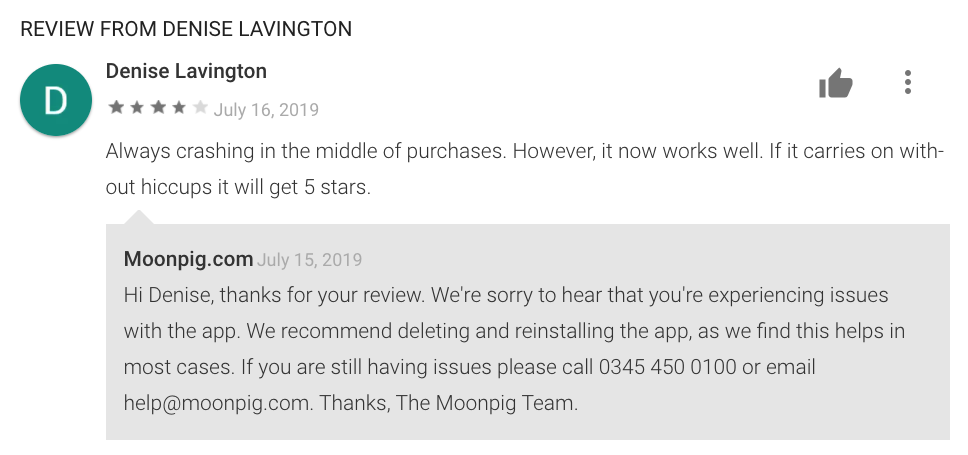
\includegraphics[width=0.44\textwidth]{images/google-play/Denise-Lavington-Review-moonpig-crashing-2019.png}
  %\end{center}
  \caption[Moonpig: User Review in Google Play `Always crashes...']{Moonpig: User Review `Always crashing in the middle of purchases'}
  \label{fig:gp-review-denise-lavington-always-crashes}
\end{wrapfigure}

As a concrete example, for the Moonpig Android app, on \nth{16} July 2019, Denise Lavington provided a review of the Android app and awarded the app four stars. The review said: \emph{``Always crashing in the middle of purchases. However, it now works well. If it carries on without hiccups it will get 5 stars."} Figure \ref{fig:gp-review-denise-lavington-always-crashes} shows the review in context in Google Play~\footnote{The review is currently still available online (\href{https://play.google.com/store/apps/details?id=com.commonagency.moonpig.uk&reviewId=gp\%3AAOqpTOH68VB5eWqnu7UAqcC81_rbOfWl6dzL_g48jrg0T40MPWBkMxe01KjStXZF6F57nxZxQa-AqosRKDd1xQ}{here}) in Google Play, two years after it was written.}.

The developer investigated this reported issue and could not find any crash in Firebase or Android Vitals that might affect purchases. A possible reason for why the crash did not appear in Android Vitals is that the underlying data is only provided by a user's device if they've opted-in to automatically providing their usage and diagnostics data~\citep{google_play_view_crashes_and_anr_errors} \textit{and} if the aggregate data exceeds an undocumented threshold (a topic discussed elsewhere in the thesis). 

Monitoring reviews can be useful to identify issues (a topic discussed in the Literature). In this case there was insufficient evidence to corroborate the user's report.

\newthought{Concommittant variation} establishes a clear connection between an action and one or more outcomes where there are no other know explanations or sources of actions that have led to those outcomes~\citep[pp. 260-266]{mill1884system}. 

\newthought{Fixing crashes may be necessary but not sufficient}
One of the issues~\footnote{\url{https://jira.catrob.at/browse/CATROID-379}} and associated bug fixes~\footnote{\url{https://github.com/Catrobat/Catroid/pull/3362}} pertaining to the Pocket Code app and the hackathon~\footnote{Via \url{https://jira.catrob.at/browse/CATROID-405}} has a discussion written by one of the project leads in the Pull Request~\footnote{\url{https://github.com/Catrobat/Catroid/pull/3362\#issuecomment-541055675}}. 
He observes there are still issues where content is not downloaded however the app no longer crashes. The high crash rate was sufficient to motivate the developers to address the source of the crash in the source code, however more work was needed to fix the failures to download and apply content. In the Pull Request, the developers also discussed the ramifications of removing the visual indicators when the user triggers a download and decided to simply try to fix the crash. As the developers could not reproduce the crash they were not confident in their `fix' working.

%%%%%%%%%%%%%%%%%%%%%%%%%%%%%%%%%%
%%%%%%%%%%%%%%%%%%%%%%%%%%%%%%%%%%
% Julian to continue from here!!!!
%%%%%%%%%%%%%%%%%%%%%%%%%%%%%%%%%%
%%%%%%%%%%%%%%%%%%%%%%%%%%%%%%%%%%

\newthought{Guarding against entropy:}
One of the app-centric case studies, Moonpig, demonstrated they actively guarded against entropy through frequent, ongoing checking of the various mobile analytics services they used. They had an assigned developer on duty who was expected to check these services during the working day and action any issues or anomalies they noticed.

\newthought{Strategic improvements in code quality:}
There are several approaches which tech companies have adopted which may improve code quality, including the reliability of mobile apps. In particular `shift-left'~\footnote{See \url{https://devopedia.org/shift-left} for a clear overview.} encourages moving various development activities earlier in the software development lifecycle. According to Google Kotlin results in 20\% fewer crashes in Android apps~\citep{googleblogs2021_androids_kotlin_first_approach} which is one way to shift-left by obviating some of the causes of crashes \emph{i.e.} poor programming practices Kotlin requires developers to be explicit in the nullability of variables and parameters so some of the issues only found at runtime in Java code is found at compile time when Kotlin is used. 

Another possible improvement is to group causes of failures, for instance by the type of Exception thrown, and help find ways to obviate those Exceptions being generated in practice. Techniques such as improving development practices, explicit training and mentoring of the development team, \emph{etc}. in addition to any changes in programming languages may help achieve this aim. The developers of the Google Home app were able to reduce \texttt{NullPointerException}'s by a third through migration from Java to Kotlin~\citep{googleblogs2020_google_home_reduces_crashes_by_a_third}.
%%%%% And see
% https://developer.android.com/topic/performance/vitals/crash#prevent-crashes-null-pointer
% https://en.wikipedia.org/wiki/Shift-left_testing (weak so not cited)

And yet an important consideration for code quality is to be aware of a possible anti-pattern: conservation of energy.

\newthought{Conservation of energy}
means developers may not be willing or practically able to fix some issues, they may lack the capacity and/or the time and/or the information and/or the environment/context needed to fix particular issues. These issues are hard to fix for these developers currently.
%
Therefore, one of the strategic considerations is how to enable developers to have justified confidence they can address the more challenging issues.

\dotfill 

% The following either needs connecting to the previous material or relocating to later in this chapter where we discuss pii and ethics.
For the Catrobat case study, the project leadership saw sufficient benefits from using mobile analytics after the hackathon that they decided to also implement it in the iOS app. They subsequently reverse this decision because of the intrusive data collection collected implicitly by Firebase Crashlytics. This topic is discussed later in chapter.\pending{Add a forward reference once that material has been added.}

\subsection{What's ``good enough"? and for whom?}